\documentclass[class=report, crop=false, 12pt,a4paper]{standalone}
\usepackage{enumitem}
\usepackage{float}
\usepackage[normalem]{ulem}
\usepackage{graphicx}
\usepackage{amsmath}
\usepackage{siunitx}
\usepackage{commath}
\usepackage{tikz}
\usetikzlibrary{positioning, fit, calc}   
\tikzset{block/.style={draw, thick, text width=3cm ,minimum height=1.3cm, align=center},   
line/.style={-latex}     
}  
\begin{document}
\section{Differential analysis of fluid flow}
What do we want to know? The velocity field, pressures, densities and temperature everywhere and anytime. Hence, these will be a function of (x, y, z, t).

List of variables
\begin{center}
  \begin{tabular}{||c c c||} 
  \hline
  Variable & Type & Units \\ [0.5ex] 
  \hline\hline
  $\begin{matrix}
    \overrightarrow{U} = u \hat{i} + v\hat{j} + w\hat{k}\\
    \overrightarrow{U} = u_1 \hat{i}_1 + u_2 \hat{i}_2 + u_3 \hat{i}_3
  \end{matrix}$ & Velocity/Vector & \si{\m\per\s}\\ 
  \hline
  $p$ & Pressure/Scalar & \si{\newton\per\meter\squared} \\
  \hline
  $T$ & Temperature/Scalar & \si{\celsius} \\
  \hline
  $\rho$ & Density/Scalar & \si{\kg\per\meter\cubed} \\
  \hline
  $T = \begin{bmatrix}
    \tau_{xx} & \tau_{xy} & \tau_{xz}\\
    \tau_{yx} & \tau_{yy} & \tau_{yz}\\
    \tau_{zx} & \tau_{zy} & \tau_{zz}
  \end{bmatrix}$ & Stress Tensor & \si{\newton\per\meter\squared} \\ [1ex] 
  \hline
 \end{tabular}
\end{center}
Since we have 12 variables, we need 12 equations to describe the fluid!

From last year, we have our conservation of mass equation
$$\frac{\partial}{\partial t} \int_V \rho \dif V + \oint_S (\rho \overrightarrow{V} \cdot \hat{n} )\dif S = 0$$
\begin{figure}[H]
  \centering
  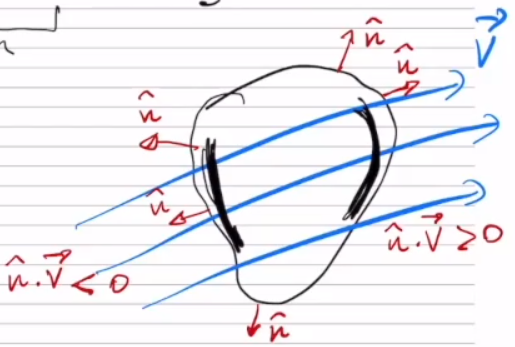
\includegraphics[width = 0.8\textwidth]{../img/euleriancontrolvolume.png}
  \caption{Consider $\hat{n}$ to be a vector coming out of the control volume. Depending on where $\hat{n}$ is, our dot product will either be greater than or less than 0.}
\end{figure}
\begin{figure}[H]
  \centering
  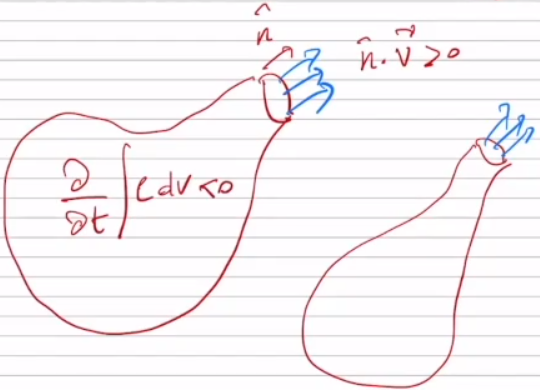
\includegraphics[width = 0.8 \textwidth]{../img/balloondeflatingeg.png}
  \caption{There is a velocity exiting the balloon. The amount of mass inside will decrease with time. The volume of the balloon will become smaller. This will be equal to the amount of mass which came out of the control volume (the balloon). If the second term of the continuity equation is positive, the first term must be negative.}
\end{figure}
\section{Conservation of mass}
Let us consider an infinitesimally small cube:
\begin{figure}[H]
  \centering
  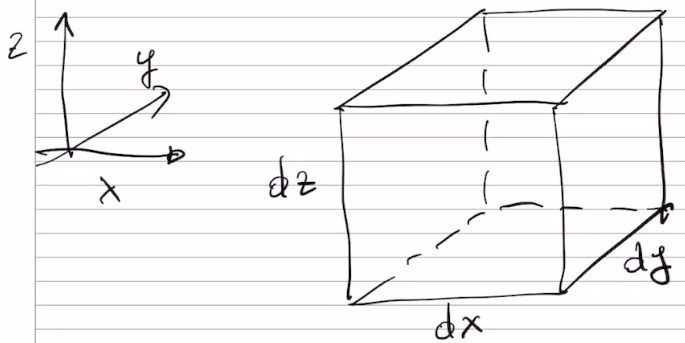
\includegraphics[width = 0.8\textwidth]{../img/infinitesimalcube.png}
\end{figure}
Consider term 1 in our continuity equation - the mass variation inside the control volume. 
$$\frac{\partial \rho}{\partial t} \cdot dV = \frac{\partial \rho}{\partial t} \cdot\dif x \cdot \dif y \cdot \dif z$$
Consider term 2 - the contribution of mass from the sides of the cube, which are orthogonal to $x$, shown below.
\begin{figure}[H]
  \centering
  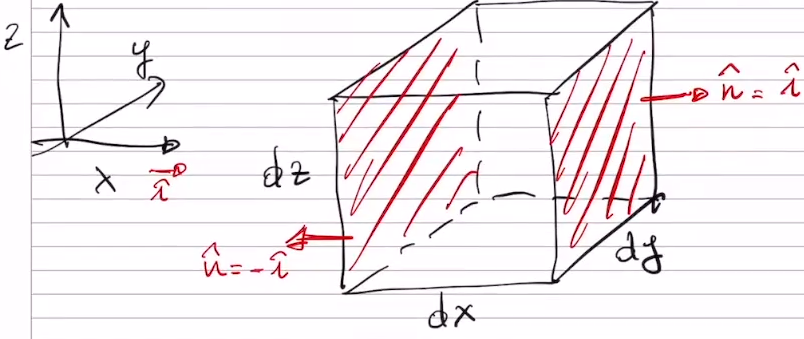
\includegraphics[width = 0.8\textwidth]{../img/infinitesimalcubewithorthox.png}
\end{figure}
Left side:
\begin{align}
  \rho \overrightarrow{V} \cdot \hat{n} \dif S &= \rho \overrightarrow{V} \cdot (-\hat{i}) \dif z \dif y\\
  &= - \rho u \dif z \dif y
\end{align}
Looking from the right side, we will not have a negative (which is coming from the fact that the normal vector is going in the opposite direction to $i$)
\begin{equation}
  (\rho u + \frac{\partial \rho u}{\partial x} \cdot \dif x) \dif z \dif y
\end{equation}
The net contribution from the orthogonal x direction is
\begin{align}
  &= (\rho u + \frac{\partial \rho u}{\partial x} \cdot \dif x) \dif z \cdot \dif y - \rho u \dif z \dif y\\
  &= \frac{\partial \rho u}{\partial x} \dif x \dif z \dif y
\end{align}
$y$ orthogonal contribution
\begin{figure}[H]
  \centering
  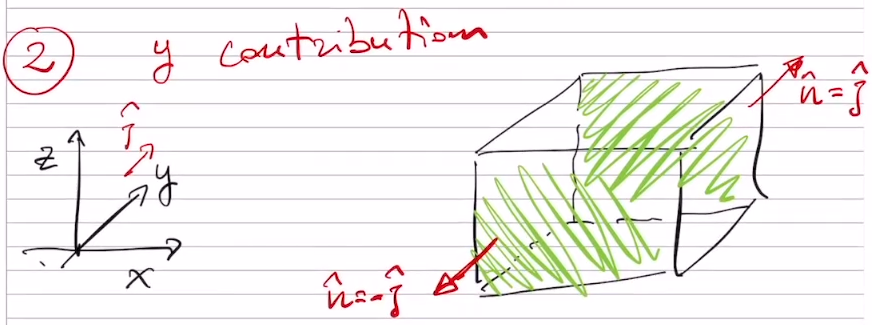
\includegraphics[width = 0.8\textwidth]{../img/infinitesimalcubewithorthoy.png}
\end{figure}
Front side
\begin{align}
  \rho \overrightarrow{V} \cdot \hat{n} \dif S &= \rho \overrightarrow{V} \cdot (- \hat{j}) \dif x \dif z\\
  &= -\rho v \dif x \dif z
\end{align}
Back side
\begin{equation}
  (\rho v + \frac{\partial \rho v}{\partial y} \cdot \dif y) \dif z \dif x
\end{equation}
Final contribution
\begin{equation}
  \frac{\partial \rho v}{\partial y} \dif y \dif z \dif x 
\end{equation}
$z$ orthogonal contribution
\begin{figure}[H]
  \centering
  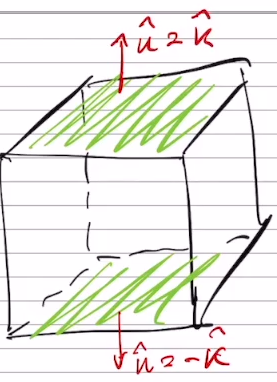
\includegraphics[width = 0.5 \textwidth]{../img/infinitesimalcubewithorthoz.png}
\end{figure}
Bottom side
\begin{align}
  \rho \overrightarrow{V} \cdot \hat{n} \dif S &= \rho \overrightarrow{V} \cdot (- \hat{k}) \dif x \dif y\\
  &= -\rho w \dif x \dif y
\end{align}
Top side
\begin{equation}
  (\rho w + \frac{\partial \rho w}{\partial z} \cdot \dif z) \dif x \dif y
\end{equation}
Final contribution
\begin{equation}
  \frac{\partial \rho w}{\partial z} \dif z \dif x \dif y 
\end{equation}
If we add up all of the contributions above, we get the conservation of mass for an infinitesimal volume.
\begin{equation}
  \frac{\partial \rho}{\partial t} \cdot\dif x \cdot \dif y \cdot \dif z + \frac{\partial \rho u}{\partial x} \dif x \dif z \dif y + \frac{\partial \rho v}{\partial y} \dif y \dif z \dif x + \frac{\partial \rho w}{\partial z} \dif z \dif x \dif y = 0
\end{equation}
This simplifies to:
\begin{equation}
  \frac{\partial \rho}{\partial t} + \frac{\partial \rho u}{\partial x} + \frac{\partial \rho v}{\partial y} + \frac{\partial \rho w}{\partial z} = 0
\end{equation}
We can simplify this a bit more by introducing a term called the divergence.
\begin{equation}
  \frac{\partial \rho}{\partial t} + \nabla \cdot (\rho \overrightarrow{V}) = 0
\end{equation}
Where $\nabla \cdot (\rho \overrightarrow{V})$ is the divergence of the vector $\rho \overrightarrow{V}$. It is a scalar.
\begin{equation}
  \frac{\partial \rho}{\partial t} + \overrightarrow{V}\cdot \nabla \rho + \rho \nabla \cdot \overrightarrow{V} = 0
\end{equation}
$\nabla \cdot \overrightarrow{V}$ is the divergence of the vector $\overrightarrow{V}$ and it is a scalar. $\nabla \rho$ is the gradient of the density $\rho$ and is a vector. It can be expanded as:
\begin{equation}
  \frac{\partial \rho}{\partial x} \hat{i} + \frac{\partial \rho}{\partial y} \hat{j} + \frac{\partial \rho}{\partial z} \hat{k}
\end{equation}
\begin{gather}
  \overrightarrow{V} \cdot \rho \nabla = (u \hat{i} + v \hat{j} + w \hat{k}) \cdot \left( \frac{\partial \rho}{\partial x} \hat{i} + \frac{\partial \rho}{\partial y} \hat{j} + \frac{\partial \rho}{\partial z} \hat{k} \right) = u \frac{\partial \rho}{\partial x} + v \frac{\partial \rho}{\partial y} + w \frac{\partial \rho}{\partial z}\\
  \rho \nabla \cdot \overrightarrow{V} = \rho \left( \frac{\partial u}{\partial x} + \frac{\partial v}{\partial y} + \frac{\partial w}{\partial z} \right)
\end{gather}
For steady flow:
\begin{equation}
  \frac{\partial \rho}{\partial t} = 0 \rightarrow \nabla \cdot (\rho \overrightarrow{V}) = 0
\end{equation}[H]
For incompressible flow, the density is constant. This means all derivatives of $\rho$ are 0. Hence, our equation reduces to:
\begin{equation}
  \rho = \textrm{const} \rightarrow \nabla \cdot \overrightarrow{V} = \frac{\partial u}{\partial x} + \frac{\partial v}{\partial y} + \frac{\partial w}{\partial z} = 0 
  \label{velocitydivergence}
\end{equation}
Each of these derivatives represent the stretch or compression of the fluid particle in the orthogonal direction. When these are all added up, it gives the variation in volume. If this is positive, it shows that the volume has increased with time. If $\rho$ is constant, then the volume cannot change. Which is why equation (\ref{velocitydivergence}) must equal 0.
\section{Conservation of momentum}
\begin{equation}
  \frac{\partial}{\partial t} \int_V \rho \overrightarrow{V} \dif V + \oint_S \rho \overrightarrow{V}(\overrightarrow{V} \cdot \hat{n}) \dif S = \sum \overrightarrow{F}
\end{equation}
We have two types of external force that can act on our infinitesimal fluid element, \textbf{volumetric} forces (e.g. gravity) and \textbf{surface} forces (shear, pressure).

Momentum is a vector as we have to take into account momentum in 3D (first term). We want to know how these change with time. The second term looks at the flux of momentum through the sides of the control volume. In this example, we are only looking at the momentum in the x direction. 
\begin{figure}[H]
  \centering
  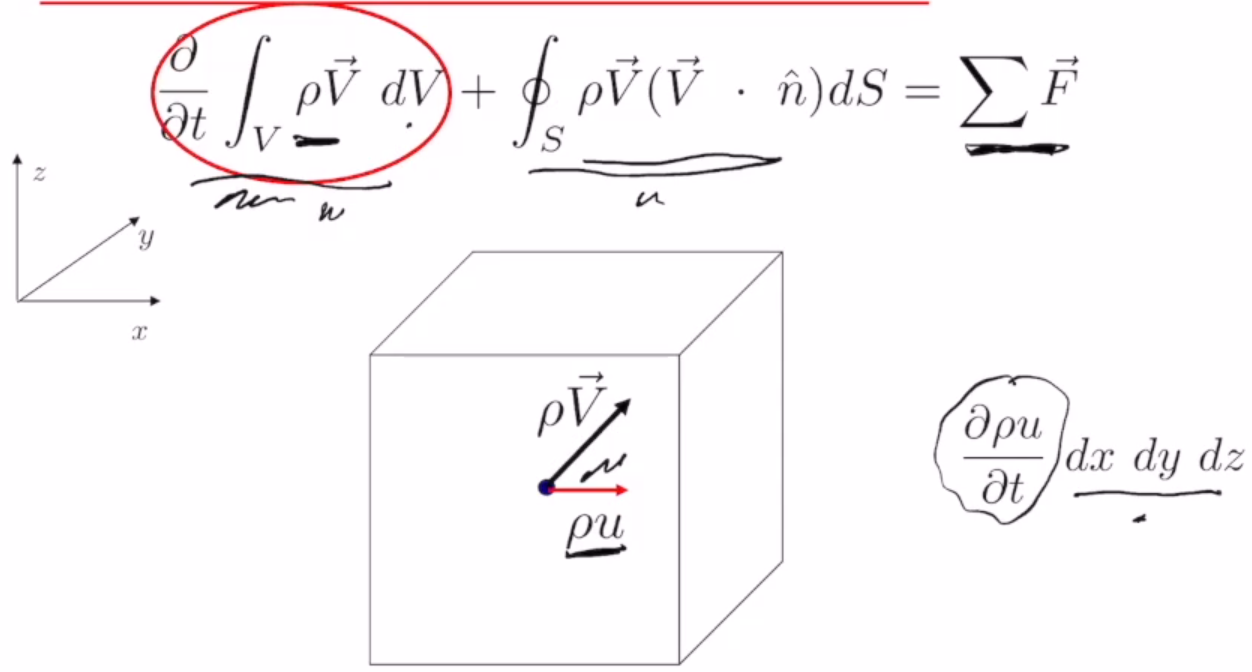
\includegraphics[width = 0.8 \textwidth]{../img/momentuminx.png}
\end{figure}
Where $\frac{\partial \rho u}{\partial t} \dif x \dif y \dif z$ is the momentum in x.
\begin{figure}[H]
  \centering
  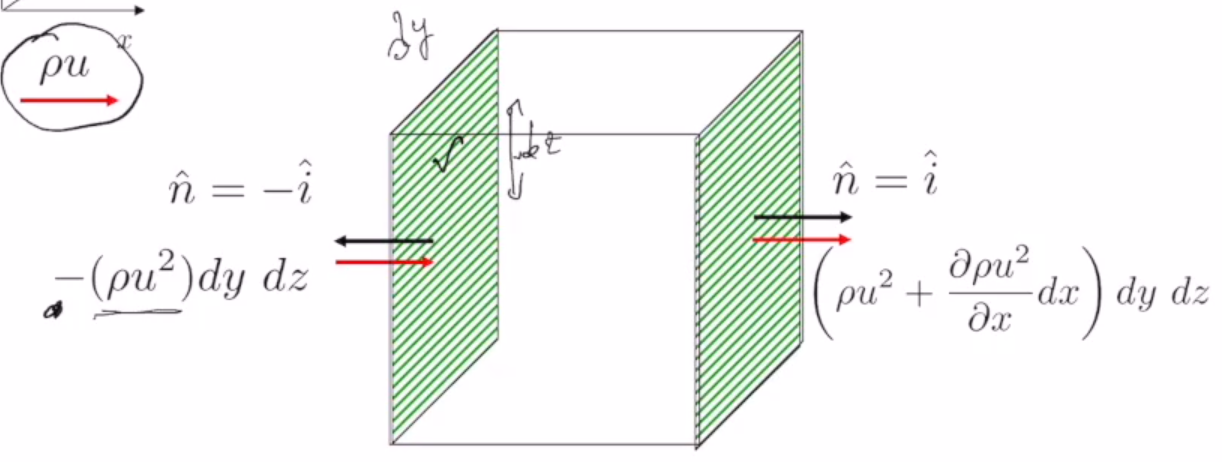
\includegraphics[width = 0.8 \textwidth]{../img/fluxinx.png}
\end{figure}
Adding the left and the right sides, we get
\begin{equation}
  \rho u (\overrightarrow{V} \cdot \hat{n}) \dif S = \frac{\partial (p u^2)}{\partial x} \dif x \dif y \dif z
\end{equation}
\begin{figure}[H]
  \centering
  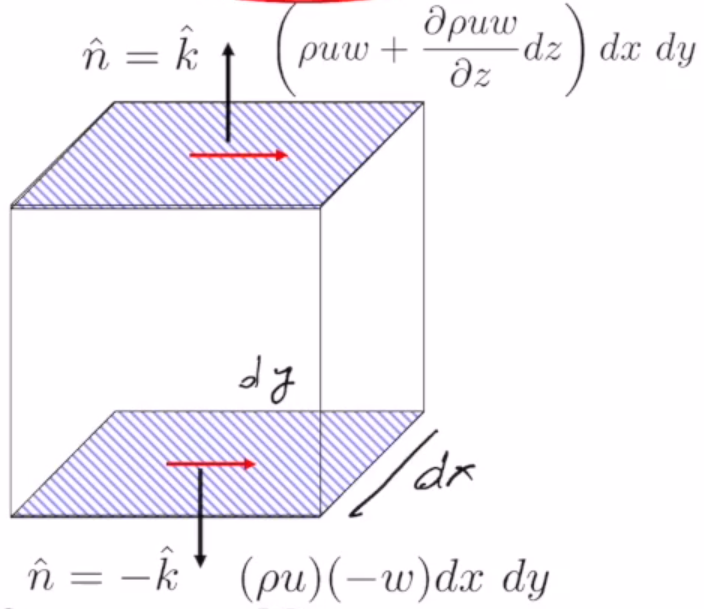
\includegraphics[width = 0.6 \textwidth]{../img/fluxthroughxy.png}
\end{figure}
Adding the net contribution to our equation:
\begin{equation}
  \rho u (\overrightarrow{V}\cdot \hat{n}) \dif S = \frac{\partial(\rho u^2)}{\partial x} \dif x \dif y \dif z + \frac{\partial (\rho u w)}{\partial z} \dif x \dif y \dif z
\end{equation}
$y$ orthogonal
\begin{figure}[H]
  \centering
  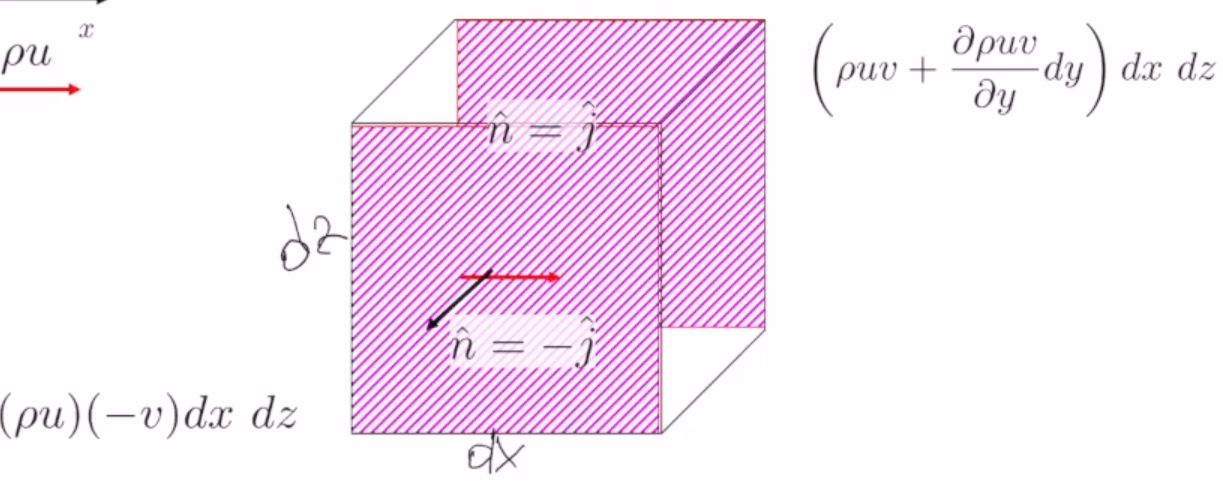
\includegraphics[width = 0.8 \textwidth]{../img/fluxthroughxz.png}
\end{figure}
Adding the net contribution to our equation:
\begin{equation}
  \rho u (\overrightarrow{V}\cdot \hat{n}) \dif S = \frac{\partial(\rho u^2)}{\partial x} \dif x \dif y \dif z + \frac{\partial (\rho u w)}{\partial z} \dif x \dif y \dif z + \frac{\partial \rho u v}{\partial y} \dif x \dif y \dif z
\end{equation}
Let us look at the $\sum \overrightarrow{F}$ term. Pressure is always exerted orthogonal to a face. We also have our $\tau$ stresses acting orthogonally
\begin{figure}[H]
  \centering
  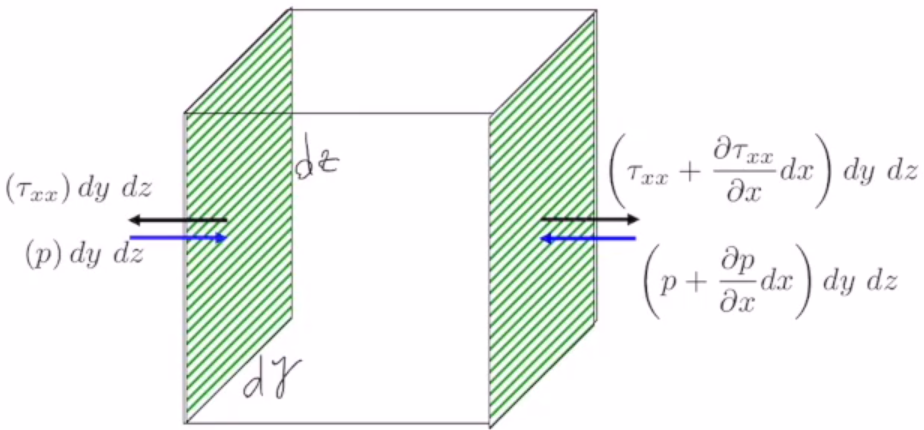
\includegraphics[width = 0.6 \textwidth]{../img/forcesinx.png}
\end{figure}
\begin{equation}
  \sum F_x = - \left( \frac{\partial p}{\partial x} \right) \dif x \dif y \dif z + \left( \frac{\partial \tau_{xx}}{\partial x} \right) \dif x \dif y \dif z
\end{equation}
z orthogonal shear force.
\begin{figure}[H]
  \centering
  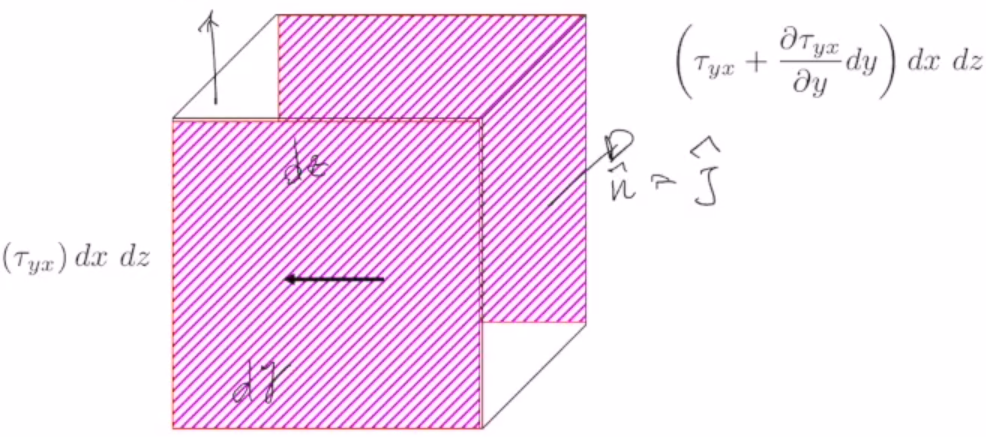
\includegraphics[width = 0.6 \textwidth]{../img/forceinxz.png}
\end{figure}
\begin{equation}
  \sum F_x = - \left( \frac{\partial p}{\partial x} \right) \dif x \dif y \dif z + \left( \frac{\partial \tau_{xx}}{\partial x} \right) \dif x \dif y \dif z + \left( \frac{\partial \tau_{zx}}{\partial z} \right) \dif x \dif y \dif z
\end{equation}
y orthogonal shear force
z orthogonal shear force.
\begin{figure}[H]
  \centering
  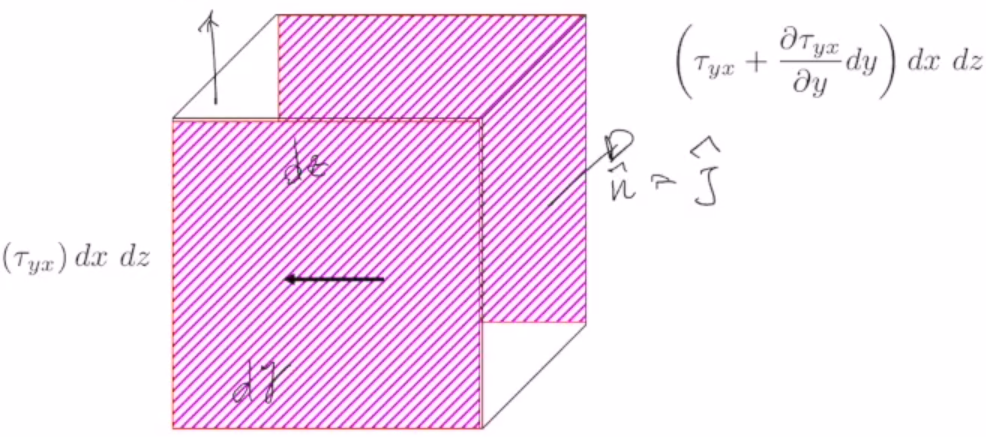
\includegraphics[width = 0.6 \textwidth]{../img/forceinxz.png}
\end{figure}
\begin{multline}
  \sum F_x = - \left( \frac{\partial p}{\partial x} \right) \dif x \dif y \dif z + \left( \frac{\partial \tau_{xx}}{\partial x} \right) \dif x \dif y \dif z + \\ \left( \frac{\partial \tau_{zx}}{\partial z} \right) \dif x \dif y \dif z + \left( \frac{\partial \tau_{yx}}{\partial y} \right) \dif x \dif y \dif z
\end{multline}
Substituting this back into our original equation, the conservation of momentum in the x direction is:
\begin{equation}
  \frac{\partial}{\partial t} (\rho u ) + \frac{\partial}{\partial x} (\rho uu) + \frac{\partial}{\partial y} (\rho uv) + \frac{\partial}{\partial z} (\rho uw) = -\frac{\partial p}{\partial x} + \frac{\partial \tau_{xx}}{\partial x} + \frac{\partial \tau_{yx}}{\partial y} + \frac{\partial \tau_{zx}}{\partial z}
\end{equation}
y direction:
\begin{equation}
  \frac{\partial}{\partial t} (\rho v ) + \frac{\partial}{\partial x} (\rho vu) + \frac{\partial}{\partial y} (\rho vv) + \frac{\partial}{\partial z} (\rho vw) = -\frac{\partial p}{\partial x} + \frac{\partial \tau_{xy}}{\partial x} + \frac{\partial \tau_{yy}}{\partial y} + \frac{\partial \tau_{zy}}{\partial z}
\end{equation}
z direction (we add $\rho g$ here due to the gravitational force acting downwards).
\begin{equation}
  \frac{\partial}{\partial t} (\rho w ) + \frac{\partial}{\partial x} (\rho wu) + \frac{\partial}{\partial y} (\rho wv) + \frac{\partial}{\partial z} (\rho ww) = -\frac{\partial p}{\partial x} - \rho g + \frac{\partial \tau_{xz}}{\partial x} + \frac{\partial \tau_{yz}}{\partial y} + \frac{\partial \tau_{zz}}{\partial z}
\end{equation}
These can be added to find that we arrive with two terms, one being the continuity equation, which must equal 0. To summarise, we have our continuity equation and momentum equations below.

Conservation of mass
\begin{equation}
  \frac{\partial \rho}{\partial t} + \nabla \cdot (\rho \overrightarrow{V}) = \frac{\partial \rho}{\partial t} + \frac{\partial \rho u}{\partial x} + \frac{\partial \rho v}{\partial y} + \frac{\partial \rho w}{\partial z} = 0
\end{equation}
x direction momentum
\begin{equation}
  \rho \left( \frac{\partial u}{\partial t} + u \frac{\partial u}{\partial x} + v \frac{\partial u}{\partial y} + w \frac{\partial u}{\partial z} \right) = -\frac{\partial p}{\partial x} + \frac{\partial \tau_{xx}}{\partial x} + \frac{\partial \tau_{yx}}{\partial y} + \frac{\partial \tau_{zx}}{\partial z}
\end{equation}
y direction momentum
\begin{equation}
  \rho \left( \frac{\partial v}{\partial t} + u \frac{\partial v}{\partial x} + v \frac{\partial v}{\partial y} + w \frac{\partial v}{\partial z} \right) = -\frac{\partial p}{\partial x} + \frac{\partial \tau_{xy}}{\partial x} + \frac{\partial \tau_{yy}}{\partial y} + \frac{\partial \tau_{zy}}{\partial z}
\end{equation}
z direction momentum
\begin{equation}
  \rho \left( \frac{\partial w}{\partial t} + u \frac{\partial w}{\partial x} + v \frac{\partial w}{\partial y} + w \frac{\partial w}{\partial z} \right) = -\frac{\partial p}{\partial x} -\rho g + \frac{\partial \tau_{xz}}{\partial x} + \frac{\partial \tau_{yz}}{\partial y} + \frac{\partial \tau_{zz}}{\partial z}
\end{equation}


\section{Stress tensor notation}
To identify a stress component we use a double subscript notation (tensor notation). The first subscript indicates the direction of the normal to the plane on which stress acts. Second subscript indicates the direction of the stress. Thus, the symbol $\tau_{ij}$ denotes a stress in $j$ direction on a face normal to the $i$-axis.
\begin{figure}[H]
  \centering
  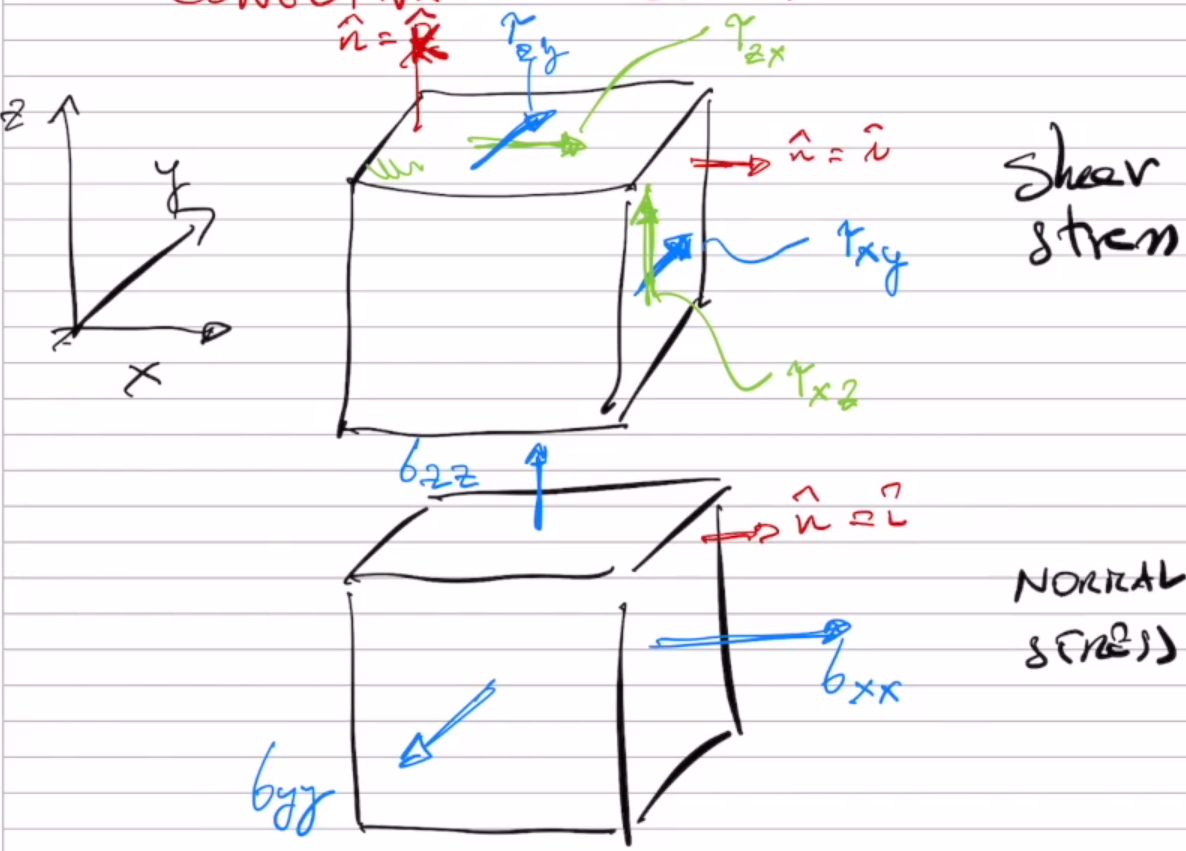
\includegraphics[width = 0.8 \textwidth]{../img/tensorforces.png}
\end{figure}
The normal stresses two contributions are pressure $p$ and viscous stress $\tau$. Pressure is always negative due to it acting against the surface (if we take the arrow coming out of the surface as positive). $\tau$ accounts for the extra stress coming from viscosity.
\begin{gather}
  \sigma_{xx} = -p + \tau_{xx}\\
  \sigma_{yy} = -p + \tau_{yy}\\
  \sigma_{zz} = -p + \tau_{zz}
\end{gather}
Parts on the opposite sides of a stress tensor are equal.
$$ \tau_{xy} = \tau_{yx}, \ \tau_{xz} = \tau_{zx}, \ \tau_{yz} = \tau_{zy} $$
\end{document}